\documentclass{ltjsarticle}
\usepackage{luatexja}
\usepackage{amsmath,amssymb}
\usepackage{graphicx}

\title{第5回：動画像処理演習1\\Optical Flow推定システムの実装}
\author{学生番号：242C2100 \\ 氏名：矢野 立己}
\date{\today}

\begin{document}
\maketitle

\section{課題1：サンプルコードの実行と閾値変更時の挙動}
MathWorks公式サイトのサンプルコードを実行し、パラメータである NoiseThreshold（ノイズ除去閾値）を変更した際の結果比較を図\ref{fig:task1_compare}に示す。

閾値をデフォルトの0.009から小さく（0.001）すると、ノイズ判定が緩くなるため、背景のわずかな変化やカメラノイズに対しても矢印（フロー）が反応する。そのため、動いていない背景部分にも細かい矢印が大量に発生し、画面全体が矢印だらけになってしまう。

逆に閾値を大きく（0.05）すると、判定が厳しくなり、はっきりとしたエッジやコントラストがある部分以外は動きが0とみなされる。ノイズは消えるが、実際に動いている部分の矢印も消えてしまい、検出漏れが多くなる。

\begin{figure}[htbp]
    \centering
    \begin{minipage}[b]{0.32\linewidth}
        \centering
        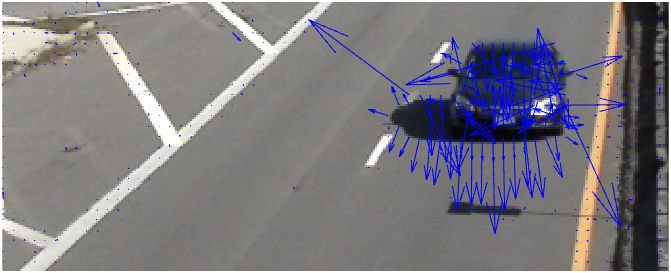
\includegraphics[width=\linewidth]{task1_result_low.png}
        \caption{閾値: 0.001 (低)}
        \label{fig:low}
    \end{minipage}
    \hfill
    \begin{minipage}[b]{0.32\linewidth}
        \centering
        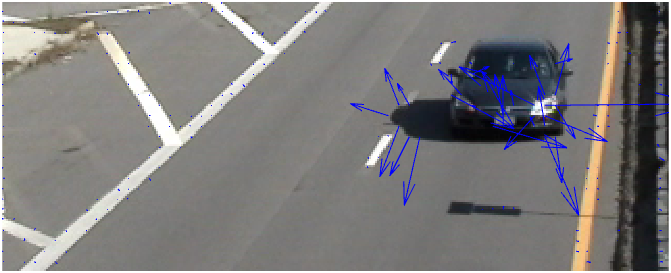
\includegraphics[width=\linewidth]{task1_result.png}
        \caption{閾値: 0.009 (標準)}
        \label{fig:default}
    \end{minipage}
    \hfill
    \begin{minipage}[b]{0.32\linewidth}
        \centering
        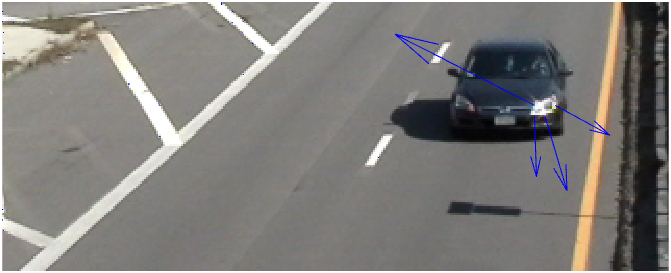
\includegraphics[width=\linewidth]{task1_result_high.png}
        \caption{閾値: 0.05 (高)}
        \label{fig:high}
    \end{minipage}
    \caption{閾値変更時のオプティカルフロー比較}
    \label{fig:task1_compare}
\end{figure}

\section{課題2：USBカメラ映像に対するオプティカルフローの算出}
入力ソースをビデオファイルからUSBカメラ（webcam）に変更し、指定された300フレームでループを終了するように変更したコードを以下に示す。

\begin{verbatim}
cam = webcam();
opticFlow = opticalFlowLK('NoiseThreshold',0.009);
h = figure; movegui(h);
hViewPanel = uipanel(h,'Position',[0 0 1 1],'Title','Plot of Optical Flow Vectors');
hPlot = axes(hViewPanel);

for i = 1:300
    frameRGB = snapshot(cam);
    frameGray = im2gray(frameRGB);
    flow = estimateFlow(opticFlow,frameGray);
    imshow(frameRGB)
    hold on
    plot(flow,'DecimationFactor',[5 5],'ScaleFactor',10,'Parent',hPlot);
    hold off
    pause(10^-3)
end
clear cam;
\end{verbatim}

実行結果を図\ref{fig:task2}に示す。

\begin{figure}[htbp]
    \centering
    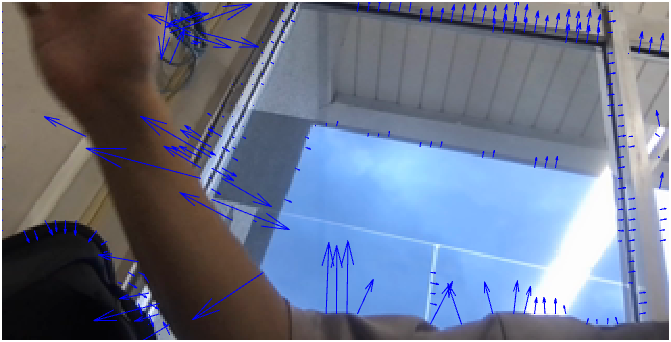
\includegraphics[width=0.7\linewidth]{task2_result.png}
    \caption{課題2の実行結果（手の動き）}
    \label{fig:task2}
\end{figure}

\section{課題3：局所領域における外れ値の影響とその対処法}
LK法は「局所領域の中のピクセルは全部同じ動きをする」という前提で計算している。しかし、動いている物体の境界部分や、光の反射による急な明るさの変化があると、領域の中に違う動きのピクセル（ノイズ）が混ざってしまい、これが外れ値になる。
LK法は最小二乗法で解いているため、このような外れ値（ノイズ）が一部でもあると、計算結果全体が大きく引っ張られて歪んでしまい、実際の動きとは全く違うデタラメな矢印が描画されてしまう。

対策としては、最小二乗法の代わりにRANSACやM推定といった外れ値に強い手法を使うことや、領域の中心に近いピクセルの重みを大きくする重み付き最小二乗法を使うこと、あらかじめ画像をガウシアンフィルタ等でぼかしてノイズを減らしておく前処理などが挙げられる。

\section{課題4：グローバル法によるオプティカルフロー推定}
画像全体の動きをまとめて計算するグローバル法の代表例として、Horn-Schunck（HS）法がある。

HS法では、局所的に解くLK法とは違い、画像全体で動きの「滑らかさ」のバランスを取るようにエネルギー関数を最小化する。エネルギー関数 $E$ は以下の式で定義される。

\begin{equation}
E = \iint \left( (I_x u + I_y v + I_t)^2 + \alpha^2 (\|\nabla u\|^2 + \|\nabla v\|^2) \right) dx dy
\end{equation}

この式は、左側の「明るさが変化しないこと（輝度不変）」と、右側の「隣り合うピクセル同士の動きが滑らかに繋がること（平滑化拘束）」の2つの条件の足し算になっており、$\alpha$ でそのバランスを調整して反復計算で解く。

この手法では、輝度不変のほかに「速度場は画像全体で滑らかに変化する」という仮定（平滑化拘束）を置いている。これにより、LK法では動きを検出できないエッジのない平坦な部分（テクスチャのない領域）でも、周囲のピクセルの動きが伝わってくるため、画像全体のフローを綺麗に補間して推定できるのが特徴である。

\end{document}
